\documentclass[aspectratio=169,11pt]{beamer}

\usetheme{Madrid}
\usecolortheme{default}
\usefonttheme{professionalfonts}
\setbeamertemplate{navigation symbols}{}
\setbeamertemplate{caption}[numbered]

\definecolor{utecblue}{RGB}{0,70,130}
\definecolor{utecwhite}{RGB}{255,255,255}
\definecolor{utecorange}{RGB}{220,105,35}
\definecolor{utecgreen}{RGB}{25,125,85}
\definecolor{utecgray}{RGB}{90,100,110}

\setbeamercolor{structure}{fg=utecblue}
\setbeamercolor{title}{fg=utecwhite}
\setbeamercolor{frametitle}{fg=utecwhite}
\setbeamercolor{block title}{fg=white,bg=utecblue}
\setbeamercolor{block body}{fg=black,bg=utecblue!7}
\setbeamercolor{alerted text}{fg=utecorange}
\setbeamertemplate{footline}{%
  \leavevmode\hbox{\begin{beamercolorbox}[wd=\paperwidth,ht=2.5ex,dp=1ex,
    center]{author in head/foot}\scriptsize
    \insertshorttitle\hspace{1em}|\hspace{1em}\insertframenumber
  \end{beamercolorbox}}%
}

\usepackage[T1]{fontenc}
\usepackage[utf8]{inputenc}
\usepackage{lmodern}
\usepackage{amsmath,amssymb,mathtools}
\usepackage{booktabs}
\usepackage{array}
\usepackage{tikz}
\usetikzlibrary{arrows.meta,positioning,calc,fit,shapes.geometric}
\usepackage{hyperref}

\newcommand{\inv}[1]{#1^{-1}}
\newcommand{\cross}{\operatorname{cross}}
\newcommand{\R}{\mathbb{R}}

\title[Tunea Tu Combi]{Tunea Tu Combi}
\subtitle{Juego de construcción y simulación física}
\author{Proyecto de Computación Gráfica}
\institute{Universidad de Ingeniería y Tecnología (UTEC)}
\date{\today}

\AtBeginSection[]{
  \begin{frame}{Hoja de ruta}
    \tableofcontents[currentsection,hideothersubsections]
  \end{frame}
}

\begin{document}

\begin{frame}
  \titlepage
\end{frame}

\begin{frame}{Hoja de ruta}
  \tableofcontents[hideallsubsections]
\end{frame}

\section{El juego}

\begin{frame}{Premisa: construir, lanzar, aprender}
  \begin{block}{Idea central}
    El jugador ensambla un vehículo con piezas, lo lanza en un nivel con
    terreno y itera sobre el diseño cuando el resultado falla.
  \end{block}

  \vspace{0.2cm}
  \begin{columns}[T]
    \column{0.5\textwidth}
    \textbf{Ciclo del jugador}
    \begin{enumerate}[label=\arabic*.]
      \item Coloca piezas en la cuadrícula.
      \item Rota, mueve y conecta componentes.
      \item Inicia la simulación y observa.
      \item Vuelve a construir y mejora.
    \end{enumerate}
    \column{0.5\textwidth}
    \textbf{Enfoque del proyecto}
    \begin{itemize}
      \item Edición basada en cuadrícula.
      \item Ensamblado procedural de física.
      \item Colisiones y restricciones en 2D.
    \end{itemize}
  \end{columns}
\end{frame}

\begin{frame}{Arquitectura general}
  \begin{center}
  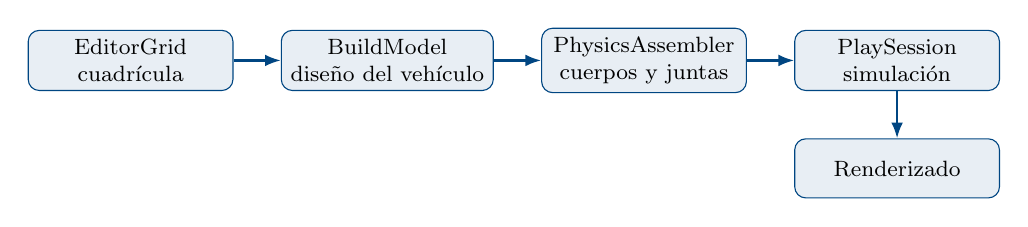
\begin{tikzpicture}[
    box/.style={draw=utecblue,rounded corners,fill=utecblue!9,
      minimum width=2.6cm,minimum height=0.75cm,align=center,font=\footnotesize},
    arrow/.style={-{Latex[length=2mm]},thick,utecblue}
  ]
    \node[box] (grid) {EditorGrid\\cuadrícula};
    \node[box,right=0.6cm of grid] (model) {BuildModel\\diseño del vehículo};
    \node[box,right=0.6cm of model] (asm) {PhysicsAssembler\\cuerpos y juntas};
    \node[box,right=0.6cm of asm] (play) {PlaySession\\simulación};
    \node[box,below=0.6cm of play] (render) {Renderizado};
    \draw[arrow] (grid)--(model);
    \draw[arrow] (model)--(asm);
    \draw[arrow] (asm)--(play);
    \draw[arrow] (play)--(render);
  \end{tikzpicture}
  \end{center}

  \vspace{0.15cm}
  \begin{itemize}
    \item La cuadrícula simplifica la interacción y mantiene la estructura.
    \item \texttt{PartDefinition} separa datos, geometría y comportamiento.
    \item El diseño es la fuente de verdad antes y durante la partida.
  \end{itemize}
\end{frame}

\section{Física}

\begin{frame}{De piezas a cuerpos rígidos}
  \begin{center}
  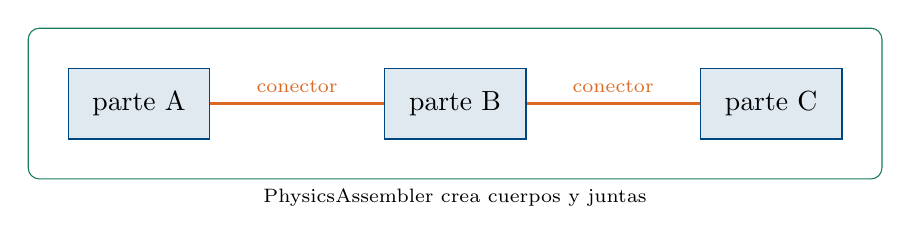
\begin{tikzpicture}[
    part/.style={draw=utecblue,fill=utecblue!12,minimum width=1.8cm,
      minimum height=0.9cm,align=center},
    arrow/.style={-{Latex[length=2mm]},thick,utecblue}
  ]
    \node[part] (a) {parte A};
    \node[part,right=2.2cm of a] (b) {parte B};
    \node[part,right=2.2cm of b] (c) {parte C};
    \draw[utecorange,very thick] (a.east)--(b.west)
      node[midway,above,font=\scriptsize] {conector};
    \draw[utecorange,very thick] (b.east)--(c.west)
      node[midway,above,font=\scriptsize] {conector};
    \node[draw=utecgreen,rounded corners,fit=(a)(b)(c),
      inner sep=0.5cm,label={[font=\scriptsize]below:PhysicsAssembler crea
      cuerpos y juntas}] {};
  \end{tikzpicture}
  \end{center}

  \vspace{0.1cm}
  \begin{itemize}
    \item Cada pieza se convierte en un cuerpo rígido (caja, círculo,
      cápsula o triángulo).
    \item Los conectores se traducen en juntas (revolute o weld).
    \item El terreno y la gravedad se definen antes de iniciar.
  \end{itemize}
\end{frame}

\begin{frame}{Detección de colisiones: AABB y SAT}
  \begin{columns}[T]
    \column{0.5\textwidth}
    \begin{block}{Broad phase: AABB}
      Descarta pares distantes comparando intervalos:
      \[
      [x_{\min}^{A},x_{\max}^{A}]\cap[x_{\min}^{B},x_{\max}^{B}]\neq\varnothing
      \]
    \end{block}
    \column{0.5\textwidth}
    \begin{block}{Narrow phase: SAT}
      Si las proyecciones en todos los ejes se solapan, las formas
      colisionan. El solapamiento mínimo da la normal y penetración.
    \end{block}
  \end{columns}

  \vspace{0.1cm}
  \begin{alertblock}{Decisión de alcance}
    AABB es simple y suficiente para el número actual de objetos. Un grid
    espacial o BVH son mejoras futuras, no requisitos faltantes.
  \end{alertblock}
\end{frame}

\begin{frame}{Fuerzas, impulsos y respuesta}
  \begin{columns}[T]
    \column{0.5\textwidth}
    \begin{block}{Respuesta por impulso}
      \[
      \Delta\mathbf{v}=\inv{m}\mathbf{P},
      \qquad
      \Delta\omega=\inv{I}\cross(\mathbf{r},\mathbf{P}).
      \]
      Un contacto transfiere momento lineal y, si es descentrado, angular.
    \end{block}
    \column{0.5\textwidth}
    \begin{block}{Fuerza sostenida vs impulso}
      \begin{itemize}
        \item Ventilador: fuerza constante mientras está activo.
        \item Vela: fuerza constante durante ventana activa (no un impulso de
          un frame), luego cooldown.
        \item TNT: impulso radial en explosión.
      \end{itemize}
    \end{block}
  \end{columns}

  \vspace{0.1cm}
  \begin{center}
    La modelación correcta de fuerzas e impulsos hace creíble el vehículo.
  \end{center}
\end{frame}

\begin{frame}{Ventilador, vela y TNT}
  \begin{columns}[T]
    \column{0.33\textwidth}
    \begin{block}{Ventilador}
      Fuerza constante persistente. Se mantiene hasta apagarlo.
    \end{block}
    \column{0.33\textwidth}
    \begin{block}{Vela de viento}
      Fuerza constante durante ventana activa ($\approx 0.75\ \mathrm{s}$),
      luego cooldown ($\approx 1.25\ \mathrm{s}$). Más intensa que el
      ventilador. Sin impulso de un solo frame.
    \end{block}
    \column{0.33\textwidth}
    \begin{block}{TNT}
      Impulso radial en explosión. Parte eliminada tras detonar.
    \end{block}
  \end{columns}

  \vspace{0.1cm}
  \begin{center}
  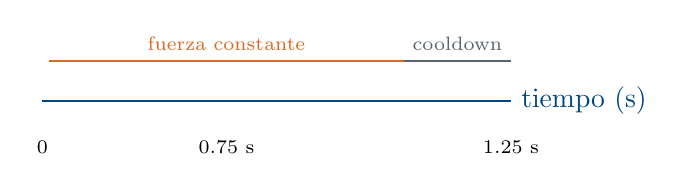
\begin{tikzpicture}[scale=0.85]
    \draw[thick,utecblue] (0,0)--(7,0) node[right] {tiempo (s)};
    \draw[thick,utecorange] (0.1,0.6)--(5.4,0.6)
      node[midway,above,font=\scriptsize] {fuerza constante};
    \draw[thick,utecgray] (5.4,0.6)--(7.0,0.6)
      node[midway,above,font=\scriptsize] {cooldown};
    \node[font=\scriptsize] at (0.0,-0.7) {$0$};
    \node[font=\scriptsize] at (2.75,-0.7) {$0.75\ \mathrm{s}$};
    \node[font=\scriptsize] at (7.0,-0.7) {$1.25\ \mathrm{s}$};
  \end{tikzpicture}
  \end{center}
\end{frame}

\begin{frame}{Juntas y estabilización}
  \begin{columns}[T]
    \column{0.5\textwidth}
    \begin{block}{Revolute}
      Bloquea la traslación entre dos anclajes, deja libre la rotación.
    \end{block}
    \column{0.5\textwidth}
    \begin{block}{Weld}
      Bloquea también el ángulo relativo. Soldadura rígida.
    \end{block}
  \end{columns}

  \vspace{0.1cm}
  \begin{block}{Corrección posicional (Baumgarte)}
    \[
      \mathbf{v}_{\mathrm{bias}}=\frac{\beta}{\Delta t}\mathbf{C},
      \qquad
      \boldsymbol{\lambda}=-K^{-1}(\mathbf{v}_{\mathrm{rel}}+
      \mathbf{v}_{\mathrm{bias}}).
    \]
    Reduce hundimiento y deriva de juntas.
  \end{block}
\end{frame}

\section{Jugabilidad}

\begin{frame}{Condición de victoria y puntuación}
  \begin{columns}[T]
    \column{0.5\textwidth}
    \begin{block}{Meta}
      Llevar partes y pasajeros a una ventana de tiempo objetivo.
      \texttt{GoalWindowTracker} detecta cuándo se cumple.
    \end{block}
    \column{0.5\textwidth}
    \begin{block}{Puntuación}
      \texttt{ScoreRules} calcula el puntaje. Los resultados se graban y
      pueden enviarse a un leaderboard.
    \end{block}
  \end{columns}

  \vspace{0.1cm}
  \begin{alertblock}{Más que una demo de física}
    Construcción, simulación, victoria y puntuación forman un sistema de
    progresión completo.
  \end{alertblock}
\end{frame}

\begin{frame}{Decisiones de diseño y futuro}
  \begin{itemize}
    \item Grid de edición: legible y evita superposiciones ambiguas.
    \item Partes basadas en datos: definiciones centralizan masa, forma y
      conectores.
    \item AABB broad phase: suficiente para el prototipo actual.
    \item Solucionador iterativo: comportamiento creíble en tiempo real.
  \end{itemize}

  \vspace{0.2cm}
  \begin{alertblock}{Trabajo futuro}
    Grid espacial o BVH cuando las escenas sean más densas. No son
    requisitos faltantes hoy.
  \end{alertblock}
\end{frame}

\begin{frame}{Conclusiones}
  \begin{block}{Mensaje principal}
    Tunea Tu Combi es un juego de construcción cuya interacción visual,
    modelo de datos, ensamblado de física y solucionador forman un solo
    pipeline:
    \[
      \text{cuadrícula} \rightarrow \text{partes} \rightarrow
      \text{cuerpos y juntas} \rightarrow \text{simulación estable}.
    \]
  \end{block}

  \vspace{0.25cm}
  \begin{center}
    \Large\textbf{¡Gracias! Preguntas}
  \end{center}
\end{frame}

\end{document}
